\chapter{Background and Related Work}
\label{chap:related}


\section{Background}

\subsection{Transactions}

The transactions in the Bitcoin network are how value is transferred between users, but they are also the value themselves.
The coins are more of an abstraction, which we can see in Satoshi Nakamoto's definition of a coin: "We define a coin as a chain of digital signatures" \cite{nakamoto2008bitcoin}.
Public key cryptography is used to control transactions; meaning a transaction is tied or owned by a public-private key pair.
To transfer the value of a transaction to another entity, the owner of the key pair locks the transaction using the public key of the recipient, and then uses their own private key to generate a signature showing that the transfer was done by the now previous owner of the transaction. The lock placed on the transaction by the previous owner makes the recipient the one in control of the transaction as they control the private key corresponding to the public one used to lock the transaction. Everyone else  can verify this transfer since the previous owner generated a signature using their private key showing that they had control of the key pair controlling the transaction at the time of the transfer. The datastructure used for transactions represents one transfer of founds from one or more previous transactions; creating a chain of signatures contained in transactions. All previous transactions within this chain can no longer be spent since they have already been transferred, so it is only the tip of the chain which are available to the owner of the key pair controlling it. However, this chain have the ability to fork and merge creating the possibility to split the value of one transaction, or merge the value of many into a single transaction. 
With the possibility of splitting value of a transaction a key pair might not control the entire value of a transaction. We should instead think of ownership of transactions outputs; which together with transaction inputs are the two main parts of a transactions. The output(s) of a transaction is where the creator of the transaction locks the value to a public key, and with multiple outputs can give different keys control of different outputs. Transaction inputs are outputs of previous transactions telling us which value the transaction transfers as shown in fig.\ref{fig:transaction}. As noted earlier, a spent transaction (output) can not be spent again since it is no longer the tip of the chain. This means that if the value given in the input(s) is not used in it's entirety in the output(s) the value missing from the output will be lost. If the creator of a transaction does not wish to transfer the entire value to another entity they can create a output which is locked to their own public key. Similarly there is no output with sufficiently large value for a transfer the sender can crate many inputs from different available outputs to reach the desired value of the transaction. 

\begin{figure}[h]  %t top, b bottom, p page | you can also use h to try to get the figure to appear at the current location
  \centering
  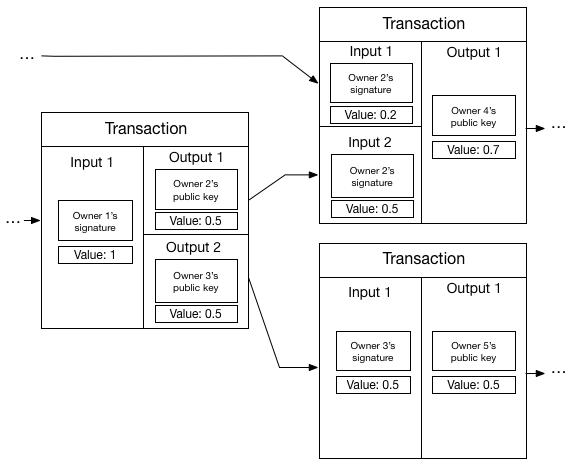
\includegraphics[width=.7\textwidth]{figures/transaction}
  \caption[Transaction chain]{A section of a example transaction chain. We see how outputs of previous transactions become inputs in new transactions and also how transactions can be split and consolidated giving us forks and merges in the chain.}
  \label{fig:transaction}
\end{figure}


\subsection{Blockchain}

The double spending problem is that a user can spend the same value twice, in this case create two transactions, each spending the same output, and both will be valid as the user signed both with their private key; the transactions might be valid but should not be accepted as they spend the same output. To avoid this in a peer-to-peer system nodes must have consensus about the transaction chain which should be public. The solution Nakamoto \cite{nakamoto2008bitcoin} proposed for creating a shared public transaction history without a central authority, is having nodes timestamp collections of transactions by hashing them together with the previous timestamp hash. 
 The structure containing the transactions at each timestamp is known as blocks, which are published to the network where each node stores their own copy. 
This process of timestamping blocks forms a chain because of the inclusion of the hash for the previous transaction collection, and thereby orders the transactions and proves their existence in relation to other transactions, also validating them futher than just the signature of the owner. A transaction included in a block is proven to have been confirmed by the network and seen as valid at a certain point and spends inputs found in transactions found in earlier blocks in the chain. If someone was to try and double spend an output they would not be able to because only one of the double spending transactions can be included in a block to maintain the integrity of the transaction chain, and if one them was included in a block and thus confirmed the other one will be seen as invalid by all nodes who have a copy of the blockchain and see that this output is already spent by the transaction included in a block. Thus the blockchain ensures consensus by nodes requiring new transactions to spend already confirmed and valid outputs found in a block, and enforcing a common transaction history.

\begin{figure}[h]  %t top, b bottom, p page | you can also use h to try to get the figure to appear at the current location
  \centering
  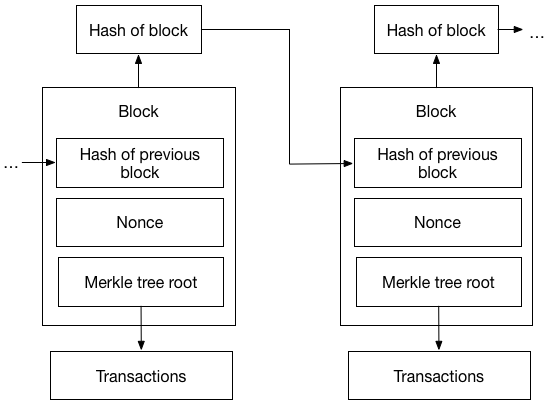
\includegraphics[width=.7\textwidth]{figures/blockchain}
  \caption[Transaction chain]{A section of a example transaction chain. We see how outputs of previous transactions become inputs in new transactions and also how transactions can be split and consolidated giving us forks and merges in the chain.}
  \label{fig:blockchain}
\end{figure}

As new transactions are created they spread around in the network, are validated, and each one node collects them in a pool for transactions that have not yet been included in a block. Nodes try to create blocks by including transactions from the pool and trying to find a nonce to include in the block such that the hash of the block starts with a given number of zero bits. This process is called mining and in addition to awarding new Bitcoin to whoever finds the solution first it requires computational power to be expended for blocks to be created. This system is called proof-of-work because the brute forcing of the hash value requires work to solve; it is also easy for others to verify the solution when the new block is published. As the blockchain grows with more blocks, the total amount of computational resources used increases. This secures the blockchain as it bolsters the immutability of blocks as they get further back from the tip, meaning they will have a greater amount of spent resources on top of them in the chain. As the Bitcoin system is a distributed one, this mining process is how nodes get to vote on their shared transaction history.
To rewrite parts of the blockchain to change the transaction history an attacker would have to redo the work from that point and exceed the height of the current used blockchain. This is because the highest chain is considered the valid one as it has the more work put into it by the nodes. The incentive of new coins when finding a solution and creating a new block also makes spending computational power to change the blockchain instead of mining less desirable. 


\subsection{Transaction Scripts}

Bitcoin transactions use a stateless, stack based, non touring complete language called script \cite{antonopoulos2017mastering}.
The outputs of transactions are locked using script by placing requirements for spending the outputs; inputs contain scripts that meet the requirements placed by their respective output scripts. The language has a predefined set of operations that can be done called Opcodes which limits possibilities of scripts. 
An example of a common locking script placed in outputs is: 
\\

OP\_DUP OP\_HASH160 <receivers public key hash> OP\_EQUALVERIFY OP\_CHECKSIG
\\

This script is a Pay to public key hash (p2pkh) script because the sender can use this script lock the output to the receivers public key hash. The receiver can spend this output by supplying their <signature> <public key> in the input which will meet the requirements placed by the output script and unlock the founds. The unlocking script will be combined with the locking script and executed to ensure that it is valid. 
\\

<receivers signature> <receivers public key> OP\_DUP OP\_HASH160 <receivers public key hash> OP\_EQUALVERIFY OP\_CHECKSIG
\\

The goal of this script is to check if the <public key> in the unlocking part hashes to the <public key hash> of the locking part, and then if the <signature> in the unlocking part matches the public key.
When the script executes the execution pointer will move left to right pushing data to the stack and do the operations specified.
In the case of P2PKH scripts the <signature> will be moved to the stack followed by the <public key>, OP\_DUP duplicates the top item on the stack, in this case the <public key>. Then the OP\_HASH160 will hash the top item of the stack meaning the top <public key>. The <public key hash> given in the locking part of the script will then be pushed to the stack and OP\_EQUALVERIFY will compare the two top items which now are the <public key hash> and the the hash of the <public key> done by the OP\_HASH operation, if they are equal they are both removed from the stack. The final operations OP\_CHECKSIG takes the two last items on the stack <public key> and <signature> and checks them to see if the signature matches the public key which means it was created with the corresponding private key.

There are two "standard" transaction types commonly used; one being pay to public key hash (P2PKH) already described, and the other is pay to script hash (P2SH) \cite{BIP16}. While users are free to create any locking script they wish within the limits of scripts, these types are recognized by most wallet software and allows for senders to transfer value by locking it in known ways. With P2PKH the receiver can just send a hash of their public key and the sender can create the locking script outlined above and just insert the hash. Instead of a public key hash P2SH allows for the same process but with complex scripts by using a hash of the script. A complex script can be created, hashed, and the hash value is used for creating the locking script resulting in:
\\

HASH160 <script hash> EQUAL
\\

The unlocking script will contain the script that was used to create the hash as one stack item only. When this is executed the whole original script, known as the redeem script will be pushed to the stack, then hashed using OP\_HASH, the script hash from the unlocking script is then pushed to the stack, and finally the two hashes are compared.
\\

<redeem script> HASH160 <script hash> EQUAL
\\

This hashing and comparing will ensure that the script supplied must be the original one. After it is confirmed that the given script is the correct one, that script itself is executed to see if it evaluates to true. The conditions for the redeem script must also be satisfied meaning that potential signatures or other data must also be supplied in the input unlocking a output. This "standard" has two executions, one being to check if the redeem script given by the redeemer matches the hash in locking script, and then the redeem script itself is run.
One reason for this is to move the responsibility for supplying these script from sender to receiver. The receiver can create whatever script they wish without the need for the sender to recreate the script when forming the transaction and locking the output. The sender receives a hash of a script and can crate the standard P2SH locking script with the format given above. The receiver needs to know the script to unlock the output but the sender does not need to know the script to transfer value; it therefore makes sense to place the burden of supplying the redeem script on the receiver instead of the sender. A typical use case for P2SH is multisig scripts: 
\\

2 <public key 1> <public key 2> 2 OP\_CHECKMULTISIG
\\

These scripts require multiple signatures to be valid, meaning multiple key-pairs which implies multiple users are required to spend a output.
In the case above two signatures is required for the two keys, indicated by the number 2 before the keys and the 2 after.
This will be the redeem script which is hashed and given to the sender which creates the P2SH locking script for this hash.
The sender does not need to know the public keys required to spend the output or that it is a multisig script in the first place. The receiver however, needs to know as they are the ones who will claim the value and most likely controls (one) of the public keys required in the redeem script.

\subsection{Segregated Witness}

Segregated Witness (segwit) is a change to mainly the Bitcoin consensus layer defined in Bitcoin improvement proposal (bip) 141 and 143 \cite{BIP141}\cite{BIP143}. It changes the structure of the validating data used to verify transactions and where it is stored. As mentioned transactions outputs have a locking script and a unlocking script; the witness is the unlocking script which can be used to check the validity of the output spent. Segwit places unlocking scripts in a witness data structure which is no longer stored inside the transaction it is used to validate. One of the reasons this is done is to fix transaction malleability, which is the ability to change the transaction id (txid) of a transaction. A txid is a hash of all the properties of a transaction including the unlocking script/witness. The only malleable parts of a transaction is the unlocking script, because a transaction is unique and outputs can only be spent once. So if the choice of inputs, choice of outputs, or the value of these changes, it is no longer the same transaction.
Therefore, when the transaction has been created most of it is non malleable, but the unlocking script can be modified in different ways without invalidating the transaction. Adding operations to the unlocking scripts or zero padding numbers used can achieve this effect and change the id while transaction is for all intents and purposes the same \cite{BIP62}. With segwit the txid hash will be calculated whiteout considering the witness data and therefore remove possibilities for malleability. Since the witness data is only used to validate the transaction itself, it is not necessary to determine the state of the blockchain and can therefore become optional for lightweight nodes saving bandwidth. 

Changes in the consensus mechanism within the Bitcoin network could cause the blockchain to fork. If one set of nodes upgrades their software containing other consensus rules they would only create blocks containing transactions following those rules. Similarly the nodes using the old rules will only consider the transactions matching their specifications. The blockchain will thus split from the point which they last agreed on in two different directions each containing their separate transaction history after the split. This is known as a hard fork because of the effects it has on the network and the blockchain. Segwit was designed to avoid this by being backwards compatible with non segwit nodes. Such a change is known as a soft fork since it does not cause a hard fork. Soft forks are easier to introduce to a decentralized network because it does not require a coordinated upgrade of software. A segwit transaction ouptut is constructed such that a non segwit enabled node will interpret the output as being spendable by everyone-i.e., reedemable by a empty signature; this means a non segwit node cannot correctly validate a segwit transaction but will not consider it invalid \cite{antonopoulos2017mastering}. 

Segwit has two "standard" transaction types which mirrors the functionality the existing ones: pay to witness public key hash (P2WPKH), and pay to witness script hash (P2WSH). The main change is how the locking scripts in the outputs is structured; instead of including the script in the output there are now only a version byte with the value 0 to 16 and then 20b bytes representing the public key hash if the output is P2WPKH or 32 bytes of a script hash if the output is P2WSH. Currently only version 0 is used with the rest being reserved for future versions \cite{BIP141}. It is the length of the bytes following the version bytes which decides which type of output the script is. A example of a P2WPKH locking script is:
\\

0 <20 byte public key hash>
\\

The unlocking script is found in the witness structure which is a stack containing the required data to validate the transaction.
In the case of the P2WPKH the witness stack will contain two elements: the <signature> and the <public key> which is the same required to validate the older P2PKH transaction type. In the case of the P2WSH type the witness stack can contain a varying amount of items depending on the requirements of the redeem script. If the redeem script is a mutlisig script the stack will contain the required amount of <signatures + public keys> with the last item of the stack always being the redeem script itself.

\subsection{Payment Channels in the Lightning Network} 

\todo{intro to payment channels and LN, ref other types of payment channels}
The structure and function of the Payment channels discussed in this section will be as they are described in the Lightning network paper by \todo{add ref}. These channels provide the means of connecting two parties, allowing them to transafer value, and with other users create a network of such channels. A payment channel is used to facilitate two people keeping track of how founds is distributed amongst themselvs. In practice this means that the parties in the channel can transfer founds to each other without broadcasting it to everyone else as is usually done in the Bitcoin system. They start with a specific distrubution of value, do some transactions back and fourth, and when they are finished they only broadcast the resulting distribution and not all the intermediary transactions-e.g., Alice and Bob have a channel with a value of 1 one coin, with the initial distrubition being 0.5 to each; Alice sends Bob 0.1 coins in three seperate transactions, resulting in a final distribution of 0.2 to Alice and 0.8 to Bob; this result is broadcast while the three 0.1 transactions are not.
In the example above we can see that the the publishing of the result only requires one transaction broadcast in comparison to three transactions if it was done outside a payment channel. All the transactions done is Bitcoin transactions because they use that standard and the value used it Bitcoin, but the ones not broadcast is off-chain, and the ones which are is on-chain transactions.
While payment channels allow for multiple transactions to be done off-chain, they do require some on-chain transactions for anchoring the channel to the blockchain. This allows for the participants to have a common starting point for the channel with a set value and distribution as well as closing a channel and distributing the value in it.
The transaction type used for this purpose is the multisig transaction we brefly discussed previously. It has a redeem script in the form of \todo{add ref to bolt rfc}:
\\

2 <public key 1> <public key 2> 2 OP\_CHECKMULTISIG
\\

The first number indicates the required number of signatures to be valid and the last number tells us the number of keys which potentially can be used for this signing. As shown above we have two required signatures and two potential keys, meaning all keys that can be used must sign. This makes it a 2of2 multisig script when we denote it in the form of $n$of$m$ where the number $n$ is the required and $m$ is the potential number of keys. The use 2of2 mutlisig scripts means that the transactions done requires the signatures of both parties in the channel ensuring they must both agree to be able to spend outputs and create new transactions.
A channel is initiated by creating a founding transaction which locks a output of that transaction with the 2of2 multisig script described above, meaning they now control that output collectively. It also creates a starting point for the channel reqorded on the blockchain allowing further transactions to be done in relation to the channel. Now the parties can do off-chain transactions until the a closing transaction is published to the blockchain; it spends the output of the founding transaction, requiring both parties signatures, which distributes the value between the parties, reflecting the off-chain transactions done.
To avoid the value of the channel being stuck in the founding transaction because one or both parties are uncooperative, because spending the founding output and thereby closing the channels requires both their signatures, a closing transaction which refunds the value is created before the founding transaction such that either party have the ability to close out the channel. The process of setting up a channel consists of the parties creating a founding transaction with a 2of2 mutlsiig output which will be the output for the channel, but they will not exchange signatures for this transaction. Then they will crate the refund transacting spending the output from the unpublished founding transaction. The exchange of signatures is done in a specific order where first the refund transaction is signed by both sides, and only then are signatures exchanged for the founding transaction, and it is published to the blockchain. The starting point of the channel is now established; containing the total value available in the channel and also allowing for refunds initiated by either party by publishing the refund transaction closing the channel. 
\\

The off-chain transactions done before the channel is closed which describes the value distribution between Alice and Bob is known as a commitment transaction. Balance or distribution in the context of payment channels is how the total value of the channel that will be split between the parties. Each time a transfer is done inside the channel a new commitment transaction is created reflecting the new balance between the two parties. E.g., the total value of the channel is 10 coins and the balance is 5 to Alice and 5 to Bob reflected in the most recent commitment transaction; Alice decides to send Bob 1 coin; now the balance is 4 coins to Alice and 6 to Bob and a new commitment transaction is created to reflect this change. This is shown in fig.\ref{fig:ln_commit} where we see the first commitment transaction on the left and the new on the right reflecting the transfer from Alice to Bob. We can also see that commitment transactions are created from the output of the founding transaction just as the refund transaction was. The balance in the channel is described in the output of these transactions, so these commitment transactions takes the total value of the channel in the form of the output of the founding transaction and splits it between the parties in its own outputs. The refund transaction can be said to be the first commitment transaction since it describes the initial balance in the channel. This initial balance will be whatever each party contributed to the input of the founding transaction. 
When the balance in the channel needs to be updated a new commitment transaction is created spending the output of the founding transaction again. The exchanging of founds between Alice and Bob consists of them creating new commitment transactions each time an transfer is done, which represents the new balance between the two. These commitment transactions is the off-chain transactions since they can be done without publishing them to the blockchain.


\begin{figure}[h]
    \centering
    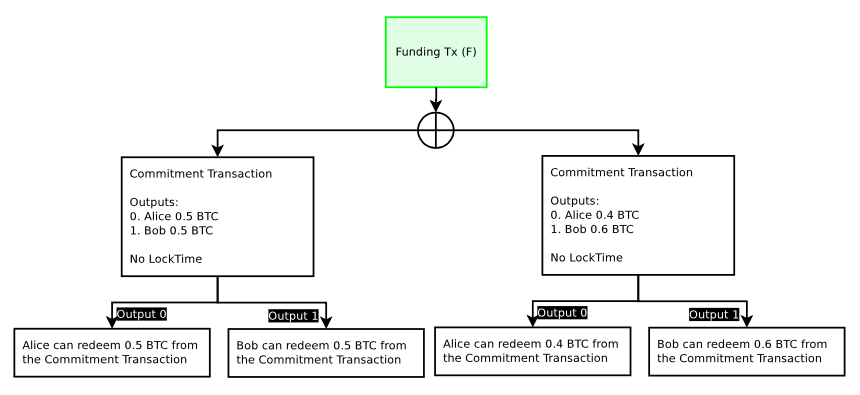
\includegraphics[width=12cm]{figures/ln_commit.png}
    \caption{Commitment transactions. Source: \cite{poon2015bitcoin}}
    \label{fig:ln_commit}
\end{figure}

\\
Alice and Bob exchanges signatures for each newly created commitment transaction.
This is satisfy the multisgnature condition on the founding transaction output used in the channel, allowing any one of them to publish the commitment transaction to the blockchain at any time if they wish. A transaction output can only be spent once, so when a commitment transaction is added to the blockchain the founding transaction is spent, and all other commitment transactions created are therefore invalid since the output they intend to spend is already used. This means that the channel no longer can be used, because its founding transaction is spent. So channels are closed out by publishing a transaction spending the output of the founding transaction. Therefore, to be able to do many transfers between the parties in the channel the commitment transactions should ideally not be published immediately. Only when something goes wrong, or both/one of the parties wishes the channel to close should the newest commitment transaction representing the current balance be published to the blockchain and thereby closing out the channel. This results in only two on-chain transactions: the founding and closing transactions, with a potential of many off-chain commitment transactions being done in-between\todo{check spelling}.
\\

A payment channel should not require the parties to trust each other to be able to transact.
The payment channels used in the Lightning Network there is mechanisms that ensures co-operation, such as the refund transaction and founding transaction creation order, which makes rendering the founds used in the channel unusable impossible. 
With the newest commitment transactions reflecting current balance in the channel, older ones will contain a different and therefore wrong balance and should therefore not be published.
Using the earlier example where a channel between Alice and Bob had the value of 10 coins and the balance was 5 to each of them. If Alice Does several payments to Bob and the balance ends up being 0 to Alice 10 to Bob, she could publish the commitment transaction where the balance was 5 to each and get all her money she send to Bob back. To deal with this problem the Lightning Channels try to penalize anyone who publishes any other commitment transaction than the latest. The penalty is that whoever published the old commitment transaction will loose all the founds to the other person in the channel.
Since both has the ability to publish a old commitment transaction we must in order to punish them find which of the two that published it; this is described in the Lightning paper as the problem of ascribing blame \todo{ref}. When the two parties exchanges signatures for a commitment transaction we in reality end up with two different versions of the same transaction. Bob signs one and sends it to Alice, and Alice signs one and sends it to Bob. This means both sides ends up with a half signed transaction which only needs their own signature before it is valid and can be published to the blockchain. The multisignature requirement means that each of them can only publish the one they received from the other.
E.g., if Bob is the one who published a commitment transaction we can find out, because he must publish one of those he received from Alice containing her signature. Because each side receivers their version of the commitment transactions from the opposing party a insurance clause can be placed on the output to the party which have the ability to publish it-i.e., when a commitment transaction is created each side makes a half signed transaction with their signature, a insurance on the output to the opposing party which means if that opposing party publishes the transaction when it is no longer the most recent, the mechanism will punish that party. This means that the commitment transactions of the two parties is not exactly the same because they will contain this mechanism, but the transaction pair will still have the same balance, spending the same outputs and have the same outputs, but the restrictions placed on those outputs will be different.
\todo{specify outputs beeing only spendable once, check also transaction section for this}
\\

The mechanism to potentially punish the party who publishes an old commitment transaction consists of timelocking their output for a some period of time meaning they cannot spend it at once, and also containing the opportunity for the the other party to spend that output if it indeed was a old commitment. Again this will result in one party getting all the founds in the channel if the other published an old commitment. The timeout of transaction outputs is done with Revocable Sequence Maturity Contracts (RSMC). When looking at the problem of ascribing blame there were two half signed copies of each commitment transaction; Bob got one where Alice has signed, and Alice one where Bob has signed. Both of them are could be published to the blockchain but only the first one will be valid, because they both spend the same output of the founding transaction. The timeout will be placed on the output to the party who publishes the transaction; reason being to try and steal from the other one would publish a transaction themselves-e.g., Alice would publish a old transaction where the balance in the channel favors her and not Bob. For each set of commitment transactions each of them will have a RSMC on the output giving founds to the holder of the commitment transaction. The output which gives founds to the other party is not encumbered with this timeout because one would not publish a old commitment transaction where the balance favors the other. 
Fig.\ref{fig:ln_timeout} shows this structure with two sets of commitment transactions and their outputs. The different colors indicate the ability for one party to publish a transaction and spend a output; Alice can broadcast the purple transactions and Bob the blue ones. The timeout is enforced by confirmations of the commitment transaction. As discussed in the \todo{ref blockchain chapter } a transaction is confirmed when included in a block. When more blocks get added on top in the chain the transactions will have more confirmations meaning the number of confirmations is is how deep a transaction is in the blockchain, so when a transaction is included in a block it has one confirmation, when another block is added to the chain it has two and so on\cite{antonopoulos2017mastering}. In the RSMC case it will make the person who publishes the commitment transaction unable to spend their output of that transaction until it has a set number of confirmations. In the paper they uses 1000 confirmations which will take a while when considering a 10 minute block interval.

\begin{figure}[h]
    \centering
    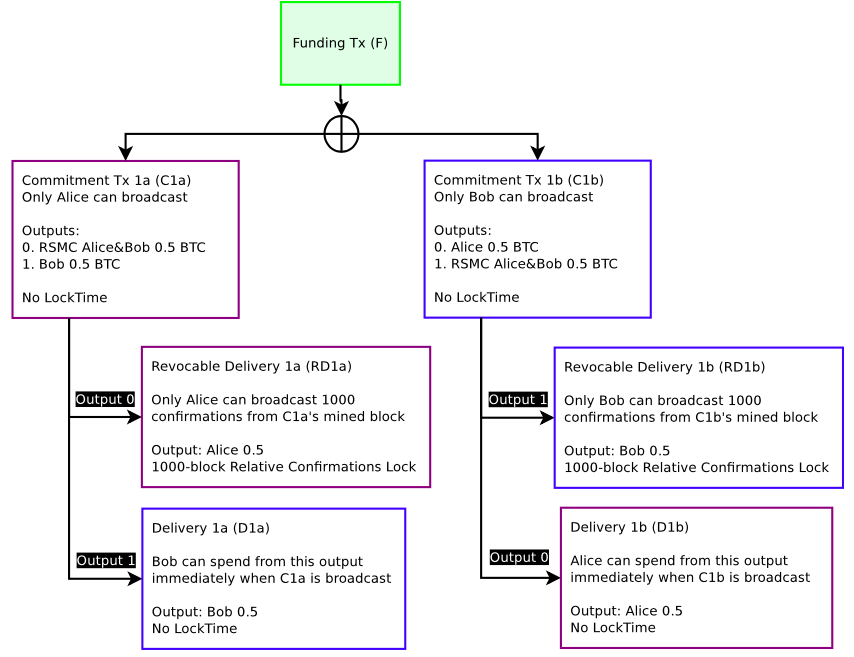
\includegraphics[width=12cm]{figures/ln_timeout.png}
    \caption{Different commitment pairs. Source: \cite{poon2015bitcoin}}
    \label{fig:ln_timeout}
\end{figure}

The need to wait for confirmations to spend the output is something that is enforced on every set of created commitment transactions. It enables the punishment of one party to spend all the founds in the channel. This punishment only applies to old commitment transactions, and therefore the punishment is only made possible when a commitment transaction pair is invalidated by creating a newer ones. This is done by creating a Breach Remedy transaction which spends the same output as the RSMC timelocked output. Each of the parties signs this transaction for the timelocked output of their own commitment transaction they want to inalidate and gives it to the other party; enabling them to spend the timelocked output belonging to the other party-e.g., Alice creates a breach remedy transaction spending her output in the old commitment transaction and sends it to Bob, and he does the same; if either of the two parties now publishes a old commitment transaction, they cannot spend their output at once because of the RSMC timelock, but the other party can publish the breach remedy transaction in addition to their own and get all founds in the channel. However, this should to be done before the timelock expires as the party which published the old commitment can now spend that output also. Both parties should therefore observe the blockchain so they can see if an old commitment transaction is published so they can use the breach remedy transaction before the timelock expires.
\todo{specify outputs beeing only spendable once, check also transaction section for this}
\\

Alice and Bob has a channel with the value of 1 coin where they both contributed 0.5 coins each. They create a funding transaction, a refund transaction (which is really the first pair of commitment transactions paying back 0.5 coins to each), sign the refund transaction and then the founding transaction. After the funding transaction is published to the blockchain the channel is ready as shown in fig.\ref{fig:ln_breach}. We can also see the current commitment transaction pair (C1a for Alice and C1b for Bob) whcih have their two outputs giving each 0.5 coins, one normal (D1b and D1b) and one timelocked Revocable delivery (RD1a and RD1b) which needs confirmations to be broadcast. Then Alice sends Bob 0.1 coins. Bob creates his breach remedy (BR1b) which spends his 0.5 of the commitment transaction (C1b); this is the same 0.5 output that used in the Revocable delivery (RD1b).
Alice does the same thing and sends it to Bob. Now that the old commitment transactions (C1a and C1b) are invalidated and they can create the updated pair (C2a and C2b) witch the new balance which outputs 0.4 to Alice and 0.6 to Bob. Now Bob decides to broadcast the old commitment transaction (C1b) to the blockchain. A strange decision since in the old balance he has 0.1 coins less but it's still a violation of the agreement in the channel of not broadcasting old commitments. 
He cannot claim his Output1 of 0.5 coins at once since he must wait for 1000 confirmations to do so because of the Revocable delivery (RD1b).
Alice sees on the blockchain that an old commitment transaction has been published. She has access to her output0 of 0.5 coins at once because it was Bob who published the commitment, so there is confirmation requirement for her. She publishes the Breach remedy transaction she received from Bob when they invalidates that commitment transaction which spends Bobs output and therefore gets the all the value in the channel. The fig.\ref{fig:ln_breach} shows this process with green indicating that a transaction is included in the blockchain and therefore invalidating all other transactions; additionally we can see how the breach remedy transactions (BR1a and BR1b) for the old commitment pair (C1a for Alice and C1b for Bob) is able to spend the same outputs as the timelocked Revocable delivery (RD1a and RD1b) crossed out with red.

\begin{figure}[h]
    \centering
    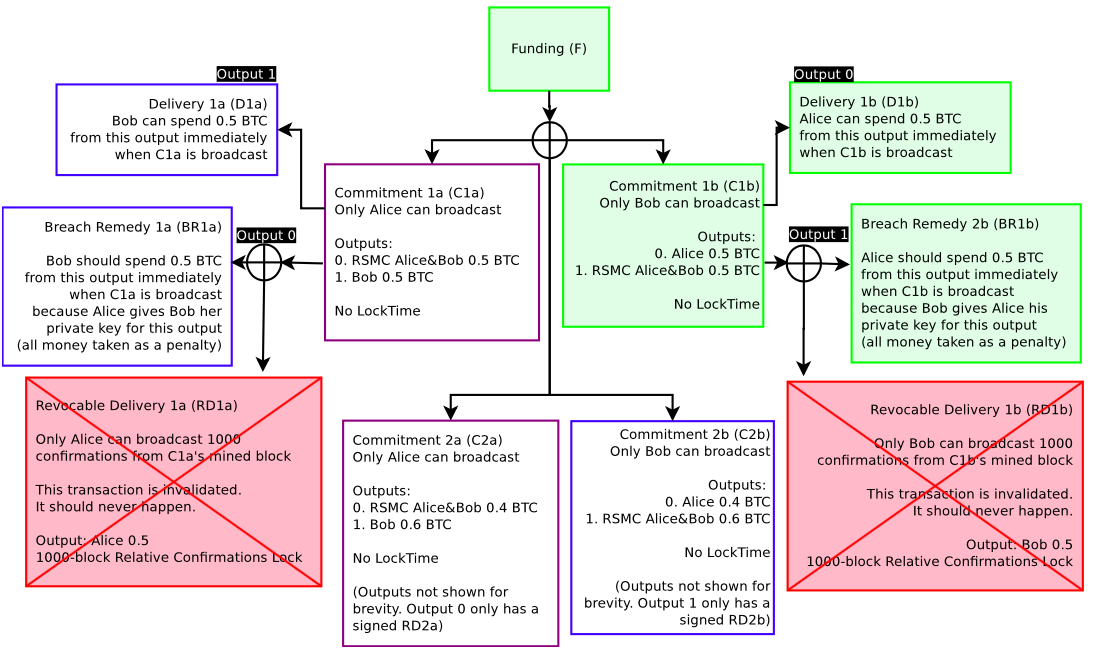
\includegraphics[width=14cm]{figures/ln_breach.png}
    \caption{Publishing old commitment transactions. Source: \cite{poon2015bitcoin}}
    \label{fig:ln_breach}
\end{figure}

Publishing a old commitment transaction as described above will spend the founding transaction and close the channel in addition to the other implications already described. If the most recent commitment is published it will also close the channel and timelock the output to the party who published it, but there will has been no Breach Remedy transaction exchanged for that commitment pair because the it has not been revoked-i.e., each party will only be able to spend their output since no agreement has been breached.
The channel can also be cooperatively closed if both parties agrees to do so. They simply create new transaction spending the founding transaction with the outputs reflecting the balance in the latest commitment. They exchange signatures and it can be published on the blockchain. This transaction does not contain any Revocable delivery transaction on its output meaning both will be able to claim their founds at once. This is because they both have to agree to close a channel this way, if they cannot agree one party can simply publish their newest commitment transaction and close the channel that way.
Closing a channel co-imperatively means that the total number of transactions published to the blockchain will be less, one founding and one closing, instead of the extra timelocked (or potential breach remedy) transactions.

\subsection{Networked Payment Channels}

The payment channels as discussed in the previous section allows for two parties to exchange founds with each other.
As mentioned earlier the LN is created by having many such interconnected channels thus forming a network. This means that a user has the ability to send founds to others across other users payment channels. If everyone needed to create a payment channel with everyone else it would not be very useful, so there are additional mechanisms that allows for payments to be routed across other users payment channels. E.g., Alice and Bob has a payment channel, but Bob and Dave also has one; Alice wishes to send founds to Dave, and she can do so by sending it first trough her existing channel with Bob, and Bob can use his channel with Dave to deliver him the payment.
As explained in the previous chapter the payment channels used in the lighting network does not require trust between the two parties in the channel. The same must be the case for doing payments across channels without trusting the intermediary nodes along the path. The construction that enables this is called Hashed Timelock Contracts (HTLC).
It creates contracts where a intermediary node have a guarantee that they can get their money from the sender, if they first transfer to the receiver. By having the intermediary nodes first pay the receiver and then get money from the sender, one stops the intermediary nodes from not passing the founds along to the receiver. If the intermediary was sent the founds first, they could simply not pay the receiver and keep the founds. However, for the intermediary nodes to accept this they need to be sure that the sender will pay them what they have already given the receiver. This is guarantee provided by the HTLC construction.
It uses a hash function with an input or preimage R; the receiver inputs R into the function and gets a hash H which is given to the sender. The sender then promises to pay the intermediary if they can provide R that generates H. The intermediary then promises to pay the receiver if they can provide a R that generates H. Now a chain of promises has been created promising to pay a amount given the condition of providing the input R which generates H. Because it was the receiver who created H and therefore has access to R they can give it to the intermediary and get the founds from them. R has now been disclosed to the intermediary, which in turn can use it to get the founds from the sender as previously promised. \todo{indicate multiple intermediaries}
\\

The promise to pay someone in exchange for disclosing R generating H is not simply a promise. It is itself a part of transactions which needs R to be valid. When the sender promises to pay the intermediary, the sender is no longer in possession of the founds because a transaction containing this clause has been created and given to the intermediary. So the founds are in a way transferred in a manner and direction one would expect (from sender to intermediary, then intermediary to receiver) but having the clause of providing R generating H to be claimed. A timelock is used to ensure that if no R is provided, the founds can be returned back to the creator of the transaction-i.e., the one who made the "promise" to pay if provided the right R. This ensures that the founds will either be delivered or returned by setting a deadline on providing R. If no such thing existed the series of transfer needed could be delayed or stopped completely by nodes not providing R.
Using an example and figures \ref{fig:htlc_promise} and \ref{fig:htlc_settle} we can see how this works in detail.
Alice wishes to send founds to Dave, but to do so she must first send them through Bob and Carol. Dave the reciver creates the hash H using the preimage R and sends H to Alice. She sees that there are tree hops for the founds to reach Dave, so she creates the first HTLC with a three day timelock and sends it to Bob shown as step 1 in fig.\ref{fig:htlc_promise}. To re-iterate the HTLC is a transaction where the preimage R has to be given for the founds to be claimed, if R is not given within the timelock timeframe (three days in this case) the founds can be reclaimed by the creator of the HTLC. Bob creates a new HTLC for Carol with the same condition except that the timelock is two days shown as step 2 in fig.\ref{fig:htlc_promise}. In step 3 Carol creates a HTLC for Dave with the timelock set to one day. At this point the founds have been sent but no one has claimed the founds from the HTLC's so the payment is not complete. If Dave does not disclose R and claim the founds from the HTLC he received it will time out, and so will eventually the other HTLC's, meaning all founds will be returned.

\begin{figure}[h]
    \centering
    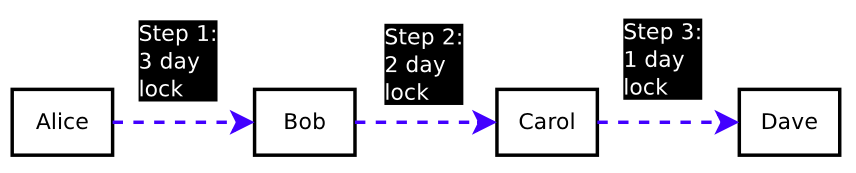
\includegraphics[width=11cm]{figures/htlc_promise.png}
    \caption{Series of HTLC's between nodes. Source: \cite{poon2015bitcoin}}
    \label{fig:htlc_promise}
\end{figure}

In fig.\ref{fig:htlc_settle} we see how the payment is completed with steps 4, 5 and 6 done. Since it is Dave who knows R he must start the process. In step 4 he reveals R to Carol to claim the founds in their HTLC. Carol can then do the same with Bob in step 5, and finally step 6 where Bob can pull his founds from Alice.
Now the founds have been fully transferred from Alice to Dave.
The reason that the timelock are shorter the closer we get to the final destination of the payment (receiver of the founds) is that it ensures that each person has time to claim the founds from the preceding one. Lets say that step 3 in fig.\ref{fig:htlc_promise} had a timelock of 5 days, and Dave waited 4 days to disclose R to Carol and get founds from her. The HTLC from Bob to Carol would have expired by then and Bob would have reclaimed his founds, meaning Carol has lost her founds to Dave without any way of getting them back.

\begin{figure}[h]
    \centering
    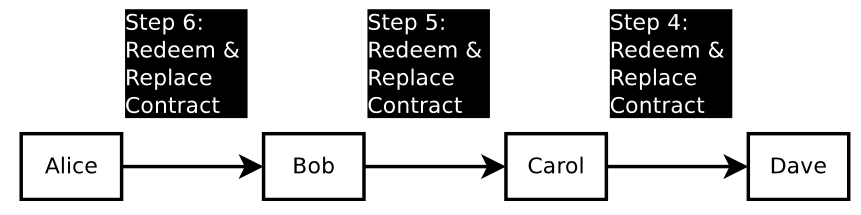
\includegraphics[width=11cm]{figures/htlc_settle.png}
    \caption{HTLC founds claimed. Source: \cite{poon2015bitcoin}}
    \label{fig:htlc_settle}
\end{figure}


\subsection{HTLC inside the payment channel}

The previous section explained the high level functioning of HTLC's and how they are used to transfer founds across different payment channels.
Here we will explain how the HTLC construct interact with the already established dynamic within a payment channel.
A HTLC inside a payment channel will be a output of commitment transactions. The outputs reflects the balance between the parties inside the channel as previously mentioned, so by having another output we can also reflect HTLC founds in transit. The HTLC output is a special type of output; it is a output script which has two different paths to redeeming the output: one is by providing the preimage R, and the other is by waiting for the timelock to expire. As with other outputs it can only be spent once, and it must be spent in one of the two ways explained.
As an output of commitment transaction the HTLC uses of founds available in the channel determined from the founding transaction. If the value of a channel is 10 coins with a 5 to each balance, a HTLC for 1 coin will be reflected in the commitment transaction as the sender of the HTLC having only 4 coins and the reciver havning 5, but the total value of the channel will still be 10 (4 sender, 1 HTLC, and 5 receiver). If they both agree on who can spend the HTLC output-e.g., receiver knows the preimage R which means the reciver can spend it, or the timelock has expired enabling the sender to spend it. If they agree on this the HTLC can be canceled by creating a new commitment transaction reflecting the new balance-e.g., using previous example the balance would be 5 to each with a normal pair of commitemnt transactions. This new balance is either the receiver getting the value of the HTLC or the sender getting it back. This is how HTLC's are resolved off-chain when the parties agree on either parties ability to spend the HTLC output, and they therefore create new commitments to reflect his.
If they cannot resolve the HTLC in this manner they can do so on-chain similarly as they could by broadcasting a commitment transaction if they cannot close the channel co-operative. 
The two ways of spending a HTLC output by providing R or waiting for the timeout is the two different types of transactions used to spend a HTLC on-chain, so Creating a "delivery" transaction which needs the preimage R to be valid or creating the "timeout" transaction which is not valid until the timelock is gone. Either one of them can be broadcasted to the blockchain and as long as it is valid it will be able to spend the HTLC ouput, but again a output can only be spent once so the first valid transaction will claim it. Because these transactions spend a output from a commitment transaction, the commitment transaction itself would also need to be broadcast on the blockchain to be able to spend its outputs. As explained earlier both parties have the opportunity to broadcast their commitment transaction but restrictions will apply when doing so. The one who published a commitment transaction had to wait before being able to claim their output, while the other party could claim theirs at once. Additionally, if the commitment transaction was an old one and had been revoked by the creation of a 
breach remedy transaction, the other party could use this to get all the founds because the broadcaster had to wait to spend their output.
The same mechanism is used when adding the HTLC output on the commitment transactions. Using the example of Alice and Bob having a 1 coin channel with a 0.5 to each balance we can see how this works. Alice sends Bob 0.1 coins using a HTLC and they create a new pair of commitment transactions (C2a, C2b) as shown in fig.\ref{fig:htlc_commit} where Alice can broadcast the purple ones and Bob the blue.


\begin{figure}[h]
    \centering
    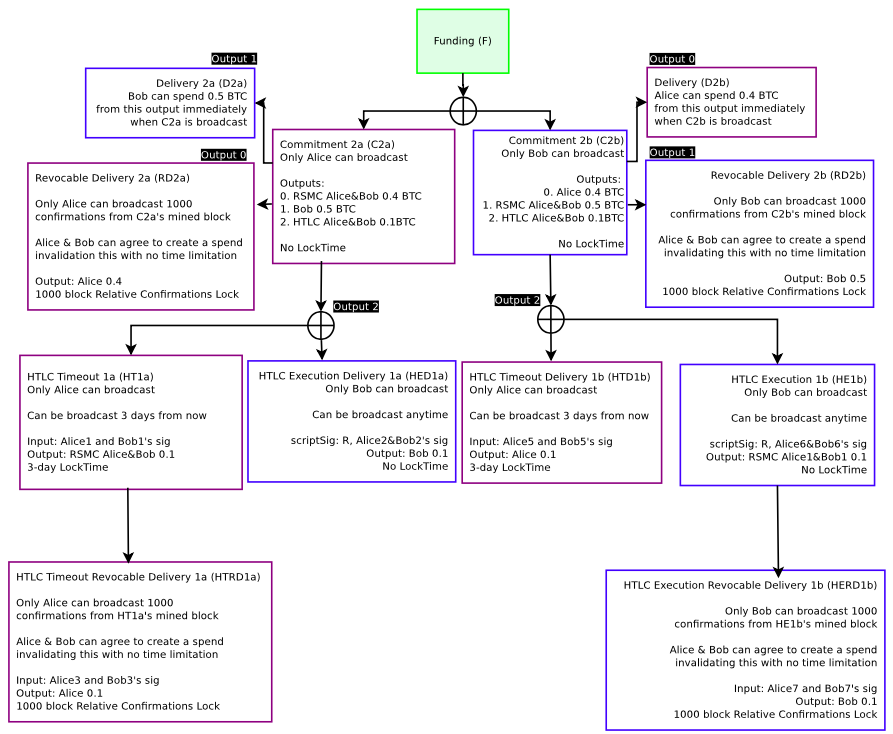
\includegraphics[width=14cm]{figures/ln_htlc.png}
    \caption{HTLC outputs in commitment transactions.  Source: \cite{poon2015bitcoin}}
    \label{fig:htlc_commit}
\end{figure}


If the sender, in this case Alice is the one who broadcasts her commitment transaction (C2a) she will have the restrictions placed on her.
In fig.\ref{fig:htlc_commit} this means that the left side will be executed. The commitment transaction (C2a) has three outputs: output0 is 0.4 to Alice herself (RD2a), but since it is her commitment transaction she will have to wait for confirmations to be able to spend; output 1 is 0.5 for Bob, which he can spend immediately (D2a); output 2 is the HTLC which has two different output paths, Bob can spend at once creating a transaction containing the preimage R (HED1a), or Alice can spend (HT1a) when the timelock has expired but this spend will have a RSMC (HTRD1a) having her wait for confirmations similarly as her normal output (RD2a). This is because similarly as old commitment transactions are invalidated by exchanging breach remedy transactions the same is done by exchanging keys for spending the HTLC output. So if an old commitment transaction is broadcast the party who broadcast will also loose the HTLC output in addition to the normal output, since the other party will be able to spend it and broadcast to the blockchain before the RSMC has enough confirmations. In this case it will enable Bob to broadcast a transaction spending the value of the HTLC before Alice can.
In the case of Bob, the receiver broadcasting the commitment transction (C2b), the left side of fig.\ref{fig:htlc_commit} will be executed. We can see that the structure is the same but now Alice and Bob have different restrictions. The output of the commitment transaction remains the same except that now it is Bob who has to wait for confirmations to get his normal output of 0.5 because of the RSMC (RD2b), and Alice can spend hers at once (D2b). In the case of the HTLC output the two parties still have their sender and receiver status meaning Alice can only spend by Timeout of the timelock (HTD1b), and Bob only by providing the preimage R (HE1b). However, since it now was Bob who broadcasted the commitment he is the one who has to get restricted getting the output by waiting for confirmations. So the output of the transaction spending the HTLC output using R (HE1b) is now a RSMC (HERD1b) which will require confirmations to become valid. This is to once again enable the other party (Alice) to get the value in the HTLC if the commitment transaction was an old one.  
\\ 

Similarly as with channel operation without HTLC it is desirable to avoid publishing to the blockchain unless it is necessary. The parties can cooperate and agree on new commitment transactions with or without HTLC outputs. To resolve a HTLC one of the parties must simply prove to the other that they are capable of spending the HTLC output and can do so on the blockchain if they wish. If Bob is the receiver he can publish the commitment transaction and if he has the preimage R he can also create a transaction spending this; because he is the broadcaster he must wait for confirmations on both but will eventually receive his founds. If Bob does not have the preimage R and the timelock has expired Alice can do the same. Since they can prove to the other party that they have this possibility they can instead just create a new commitment transaction pair with the HTLC value either transferred to Bob or returned to Alice, thereby keeping  commitment transactions off-chain and have the channel remain open. When doing this they need to invalidate their old commitment transactions and also the HTLC output of these by exchanging breach remedy transactions and keys. So again we have a system for exchanges between two parties but with the possibility of also using HTLC's which requires no trust, few transactions to be broadcast to the blockchain unless one party is unresponsive or unwilling to co-operate, and allows for founds to be transferred trough many channels.  
When using the HTLC construct to send founds across these channels as shown in fig.\ref{fig:htlc_settle} broadcasting to the blockchain as discussed in this section will ensure the transfer will finish in the event of a node not co-operating as illustrated in fig.\ref{fig:htlc_bc}.

\begin{figure}[h]
    \centering
    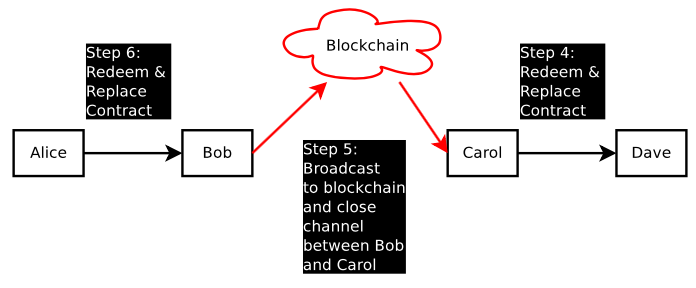
\includegraphics[width=10cm]{figures/htlc_bc.png}
    \caption{ Settlement of HTLC contracts in the event of unresponsive node using the blockchain. Source: \cite{poon2015bitcoin}}
    \label{fig:htlc_bc}
\end{figure}

\section{Related Work}

\section{Anonymity and privacy notions}


Much of the work already done with regards to blockchain analysis does not consider the LN, as most the work proceeds the inception of the LN. But the methods used, and how information is deduced from the data contained there can nevertheless be helpful for this project.
Because the blockchain is a public distributed datastructure containing all transactions done by every Bitcoin user, it is by its nature something that limits privacy. Analyzing the blockchain can theoretically give us all records of all transactions related to a single individual; this will include the amount sent and received, the time and date this was done, and which addresses these transactions was going to or coming from. However, these addresses used can be generated by users at will. Therefore it is considered best practice when using Bitcoin to generate a new address for each transaction. Doing this results in transactions between new addresses without knowing which addresses belongs to the same user of another address-i.e., there is no longer a 1-to-1 mapping between users and addresses. 
This use of new addresses for each transaction is known as Pseudonymity which is defined by by Pfitzmann and Köhntop \cite{pfitzmann2001anonymity} as: "Pseudonymity is the use of pseudonyms as IDs.". They also define pseudonymity in relation to linkability, which depending on the context has different levels of anonymity. One of these which are very relevant is the transaction pseudonym. For this context they explain that for each transaction a different pseudonym is used, like a random number. This makes different transactions pseudonyms hard to link by themselves, which will give it strong anonymity. The definition transaction pseudonyms is exactly how the Bitcoin system enables some degree of privacy to its users. Having a new pseudonym for each transaction makes it difficult for observers to link the activity of users. This relates to the privacy notion of unlinkability which is also discussed by Pfitzmann and Köhntop; it refers to the inability to find a relation between two items in a system. 
If an address is reused for several transactions it would be trivial to link these together, however, this is not the only way of linking transactions as we will discuss later. According to Pfitzmann and Köhntop unlinkability is one of three main concepts of anonymity and privacy. The other is anonymity, which is defined as such: "Anonymity is the state of being not identifiable within a set of subjects, the anonymity set."\todo{ref here because quite?}, and unobservability which means that no message is any different from random noise-i.e. encryption \todo{correct?}. The latter is not applicable to the Bitcoin system as it is a open system with a public record of messages (transactions) which is observable to the same degree by every participant. The system is also not anonymous as the subjects can be distinguished by their addresses. Pseudonymity and unlinkability is the two privacy concepts used to avoid full transparency of activity within the system. A paper by Androulaki \cite{androulaki2013evaluating} suggests some privacy notions relevant for Bitcon: activity unlinkability and user profile indistinguishability. The latter refers to the ability of a observer to link different addresses belonging to the same user revealing all their activity. This is a more specified unlikability notion describing the lack of relationship between addresses. User profile indistinguishability refers to how good anonymity is for users relating to other users. A user profile can consist of addresses or transactions which is linked meaning they are discovered as belonging to the same user. User profile indistinguishability means it should be hard for a adversary to link addresses or transactions to the right user and thereby constructing correct user profiles.

\paragraph{}
There exists work were the authors suggest different privacy notions for Bitcoin and also some for different payment networks.
One such paper that does this specifically for Bitcoin privacy is \cite{androulaki2013evaluating}. The paper did analysis on blockchain data and the notions they propose reflects this. They describe two notions called Activity unlinkability and User Profile indistinguishability. The first one refers to the ability of a adversary to link different addresses belonging to the same user. The result of linking this information is that potentially all activity of the user is revealed. While activity unlinkability describes anonymity for a single user, 

\paragraph{}
The recent paper by Malavolta et al. identifies some privacy notions specifically for payment channel networks \cite{malavolta2017concurrency}. The two notions are value privacy and relationship anonymity. Value privacy is that users outside the payment path cannot learn the value of the payment. A payment path is the route the payment travels inside the network. The notion is specified to only be off-path meaning it only considers nodes that are outside the path, so the nodes in the path will learn the value. Relationship anonymity is a more general anonymity concept which relates to likability. Pfitzmann and Köhntop \cite{pfitzmann2001anonymity} also defines this concept and explain that it relates so sender and recipient anonymity but is a weaker anonymity concept. Relationship anonymity means that the relationship between sender and receiver is unlinkable; who sends a message can be discovered and similarly who receives a message, but their relationship can not. Malavolta et al. \cite{malavolta2017concurrency} suggests that this concept is a relevant property for on-path payments in payment channel networks. This means that the nodes that are in the payment path in the network will not be able to link the sender and receiver of a payment



Therefore the goal of the studies who analyzed blockchain data was to cluster addresses used by the same individual, and negate the effect of users creating multiple addresses for different transactions \cite{herrera2015research}, and by doing this also creating user profiles that contain transaction data for that user.

One of the first studies which analyzed data from the blockchain to assess privacy was done by Reid and Harrigan \cite{reid2013analysis}.
They used the data to construct two networks, one transaction network and one user network. A Bitcoin transaction stored in the blockchain has at least one input and one output. A output of one transaction will eventually be an input on another. A network created with this transaction data will show how transactions are connected and therefore how founds are moving. The user network tries to link addresses which are likely to belong to the same user. This will create a network were we can see relations between different users. We can also see the transactions were the addresses of a particular user is involved. This clustering of addresses was done in two ways: the input addresses of a transaction with multiple inputs was assumed to be from the same user; the other way was using online sources and online Bitcoin services which had information linking multiple addresses to one user. The review paper by Herrera-Joancomart\́i\cite{herrera2015research} states that this user network model allowed Reid and Harrigan do user centered analysis, and therefore give context to the data in the blockchain.

Another paper trying to do address clustering is Androulaki et al. \cite{androulaki2013evaluating}, were they in addition to grouping multiple input addresses for a transaction to the same user, they also utilized the output. Since a single unspent output must be consumed in its entirety by a input for a new transaction, transactions will often generate change. E.g., a user has a 5 coin unspent output available and they are paying someone else 4 coins; the payment transaction will have one output with 4 to the other user, and one output back to the sender with the remaining 1 coin. The address this change is sent to is referred to in the paper by Androulaki et al. as a shadow address. It will not be the same address which was used send the payment but will be a new one belonging to the sender.
To identify which address belonged to the receiver and which is the shadow address they looked at the addresses previously used in the blockchain. The shadow address was assumed to be newly created to receive the change so if one of the output addresses had already appeared in the blockchain they assumed it to be the receiver reusing an address. They also utilized machine learning techniques to further group addresses based on behaviour. They were able to unveil 40\% of user profiles in their experiment. This accurate figure is made possible by having a ground truth, because the data used was from a simulated use of Bitcoin.

A more active approach to help clustering addresses is actively participating in the network to collect data, which was used in a study by Meiklejohn et al. \cite{meiklejohn2013fistful}. They participated in mining pools, withdrew and deposited founds on banking services or wallet services, used gambling sites, and purchased goods from vendors. Doing this they could gather addresses and because the addresses collected was certain to belong to a known entity, the tagged addresses would aid clustering in addition to the methods described earlier.
A important remark done both by Meiklejohn et al.\cite{meiklejohn2013fistful} and Reid and Herrigan \cite{reid2013analysis} is that a big entity in the network which does transactions with a large number of other users will have greater opportunity to identify or track users. Such a entity might be a exchange were people trade real money for Bitcoin, in such cases services will most likely have identifying information of users linked to their addresses.

In the LN the blockchain is used to open and close payment channels between a pair of nodes \cite{poon2015bitcoin} \cite{malavolta2017concurrency}. These payment channels between nodes form a network which is the LN itself, and were payments can be transferred between two parties without the two needing to have their own payment channel; meaning the payment is routed through the payment channels of intermediary nodes.
Herrera-Joancomartí et al. discusses in their paper \cite{herrera2016privacy} privacy in relation to Bitcoin scaling solutions and also points to several problems with blockhain analysis. One central issue is the sheer size of the blockchain. Herrera-Joancomartí et al. states that at the time of writing that paper the blockchain was 72 GB. The other papers discussed here which did blockchain analysis, did so in 2013 when the blockchain was around 8 GB; now it is over 140 GB \cite{blockchain_size}. 
Herrera-Joancomartí et al. also points out that the clustering heuristics used in previous studies \cite{reid2013analysis}  \cite{meiklejohn2013fistful} are no longer applicable when considering off-chain transactions. Also the transactions themselves that are done off-chain will not be available in the blockchain for analysis. Herrera-Joancomartí et al. suggests that using payment channel networks will increase the privacy of users with regards to blockchain analysis, but that the existing methods may be adapted to analyze the payment channels in a network such as the LN. In the LN paper \cite{poon2015bitcoin} the transaction used to open a channel is referred to as the founding transaction. The output of this transaction is used as input of the transaction closing the channel-i.e., the founding (opening) transaction and closing transaction is linkable. Furthermore, in the LN developer mailing list there is mention of the founding (here referred to as anchor) transaction can imply the network topology \cite{rusty_routing1}. This is because all channels must be anchored in the blockchain with a founding transaction signed by both parties in the channel. This possibility is also mentioned in the LN paper itself \cite{poon2015bitcoin}: by monitoring the blockchain for founding transactions a routing map of can be theoretically built. We do not know whether or not this possibility has been explored any further.

\subsection{Network Analysis}

There has been no studies doing network analysis on the LN or other payment channel networks.
However, there has been identified several factors in the LN that will impact anonymity.
Herrera-Joancomartí et al. \cite{herrera2016privacy} suggest that the typology of the LN will greatly affect privacy. 
They propose that a possible typology for the LN is one were there are some highly connected core nodes that have big capacity channels with each other, while the end users connect to one of these each when they want to do transactions. In contrast to the Bitcoin network which is a decentralized p2p network, the LN with this topology will be a more centralized one. The number of core nodes and how many connections they have will of course play a big role in the degree of centralization. But any degree of centralization with some nodes being more connected than others will likely have a effect on anonymity. These nodes may be in a position to know both source and destination of payment done in the network. Which violates the privacy notion of relationship anonymity for payment channel networks suggested by Malavolta et al. \cite{malavolta2017concurrency} discussed in section 2.1.
However, onion routing \cite{LN_onion_implementation} has been implemented for the LN which provides relationship anonymity.
In the payment path a node will only know where it received the payment from and where to forward it to. It cannot know if where it received it from was the sender or just another node in the path, or if the next node is the final receiver or just another forwarder. 

\paragraph{}
The mechanism used to transfer the payments over multiple channels in the LN is called Hashed Timelock Contract (HTLC). This contract states that the receiver must supply a preimage (input used in a hash function) to claim the founds from the contract; if this is not done within some time frame the sender will get their founds back. Each node in the path, from the sender to receiver promises to pay the next node by using the HTLC. So, a HTLC between two nodes is created for each hop in the path. The final receiver then discloses the preimage to the node before it in the path, which in turn can now get the founds from the node before it because it now knows the preimage.  This happens until the founds are pulled from the original sender. The term contract is used because if one of the nodes breaches the terms, the contract can still be enforced by using the blockchain to broadcast transaction data and close out the channel to claim the founds. In this manner two parties can transfer founds in a payment path containing untrusted intermediaries. Malavolta et al. \cite{malavolta2017concurrency} points out that this preimage is the same for each HTLC in the path for a payment, it can therefore be used as an identifier among many payments done by the nodes in the network. This means that two nodes can determine that they both where in the path of of the same payment by comparing preimage value. They also suggest that if a node in the path is uncooperative and the HTLC is enforced on the blockchain, the data broadcast there containing the preimage can be used to find the path used for the payment, even without being part of the payment path.